% Options for packages loaded elsewhere
\PassOptionsToPackage{unicode}{hyperref}
\PassOptionsToPackage{hyphens}{url}
\PassOptionsToPackage{dvipsnames,svgnames,x11names}{xcolor}
%
\documentclass[
  authoryear,
  preprint,
  3p,
  twocolumn]{elsarticle}

\usepackage{amsmath,amssymb}
\usepackage{iftex}
\ifPDFTeX
  \usepackage[T1]{fontenc}
  \usepackage[utf8]{inputenc}
  \usepackage{textcomp} % provide euro and other symbols
\else % if luatex or xetex
  \usepackage{unicode-math}
  \defaultfontfeatures{Scale=MatchLowercase}
  \defaultfontfeatures[\rmfamily]{Ligatures=TeX,Scale=1}
\fi
\usepackage{lmodern}
\ifPDFTeX\else  
    % xetex/luatex font selection
\fi
% Use upquote if available, for straight quotes in verbatim environments
\IfFileExists{upquote.sty}{\usepackage{upquote}}{}
\IfFileExists{microtype.sty}{% use microtype if available
  \usepackage[]{microtype}
  \UseMicrotypeSet[protrusion]{basicmath} % disable protrusion for tt fonts
}{}
\makeatletter
\@ifundefined{KOMAClassName}{% if non-KOMA class
  \IfFileExists{parskip.sty}{%
    \usepackage{parskip}
  }{% else
    \setlength{\parindent}{0pt}
    \setlength{\parskip}{6pt plus 2pt minus 1pt}}
}{% if KOMA class
  \KOMAoptions{parskip=half}}
\makeatother
\usepackage{xcolor}
\setlength{\emergencystretch}{3em} % prevent overfull lines
\setcounter{secnumdepth}{5}
% Make \paragraph and \subparagraph free-standing
\makeatletter
\ifx\paragraph\undefined\else
  \let\oldparagraph\paragraph
  \renewcommand{\paragraph}{
    \@ifstar
      \xxxParagraphStar
      \xxxParagraphNoStar
  }
  \newcommand{\xxxParagraphStar}[1]{\oldparagraph*{#1}\mbox{}}
  \newcommand{\xxxParagraphNoStar}[1]{\oldparagraph{#1}\mbox{}}
\fi
\ifx\subparagraph\undefined\else
  \let\oldsubparagraph\subparagraph
  \renewcommand{\subparagraph}{
    \@ifstar
      \xxxSubParagraphStar
      \xxxSubParagraphNoStar
  }
  \newcommand{\xxxSubParagraphStar}[1]{\oldsubparagraph*{#1}\mbox{}}
  \newcommand{\xxxSubParagraphNoStar}[1]{\oldsubparagraph{#1}\mbox{}}
\fi
\makeatother


\providecommand{\tightlist}{%
  \setlength{\itemsep}{0pt}\setlength{\parskip}{0pt}}\usepackage{longtable,booktabs,array}
\usepackage{calc} % for calculating minipage widths
% Correct order of tables after \paragraph or \subparagraph
\usepackage{etoolbox}
\makeatletter
\patchcmd\longtable{\par}{\if@noskipsec\mbox{}\fi\par}{}{}
\makeatother
% Allow footnotes in longtable head/foot
\IfFileExists{footnotehyper.sty}{\usepackage{footnotehyper}}{\usepackage{footnote}}
\makesavenoteenv{longtable}
\usepackage{graphicx}
\makeatletter
\def\maxwidth{\ifdim\Gin@nat@width>\linewidth\linewidth\else\Gin@nat@width\fi}
\def\maxheight{\ifdim\Gin@nat@height>\textheight\textheight\else\Gin@nat@height\fi}
\makeatother
% Scale images if necessary, so that they will not overflow the page
% margins by default, and it is still possible to overwrite the defaults
% using explicit options in \includegraphics[width, height, ...]{}
\setkeys{Gin}{width=\maxwidth,height=\maxheight,keepaspectratio}
% Set default figure placement to htbp
\makeatletter
\def\fps@figure{htbp}
\makeatother

\usepackage{booktabs}
\usepackage{longtable}
\usepackage{array}
\usepackage{multirow}
\usepackage{wrapfig}
\usepackage{float}
\usepackage{colortbl}
\usepackage{pdflscape}
\usepackage{tabu}
\usepackage{threeparttable}
\usepackage{threeparttablex}
\usepackage[normalem]{ulem}
\usepackage{makecell}
\usepackage{xcolor}
\makeatletter
\@ifpackageloaded{caption}{}{\usepackage{caption}}
\AtBeginDocument{%
\ifdefined\contentsname
  \renewcommand*\contentsname{Table of contents}
\else
  \newcommand\contentsname{Table of contents}
\fi
\ifdefined\listfigurename
  \renewcommand*\listfigurename{List of Figures}
\else
  \newcommand\listfigurename{List of Figures}
\fi
\ifdefined\listtablename
  \renewcommand*\listtablename{List of Tables}
\else
  \newcommand\listtablename{List of Tables}
\fi
\ifdefined\figurename
  \renewcommand*\figurename{Figure}
\else
  \newcommand\figurename{Figure}
\fi
\ifdefined\tablename
  \renewcommand*\tablename{Table}
\else
  \newcommand\tablename{Table}
\fi
}
\@ifpackageloaded{float}{}{\usepackage{float}}
\floatstyle{ruled}
\@ifundefined{c@chapter}{\newfloat{codelisting}{h}{lop}}{\newfloat{codelisting}{h}{lop}[chapter]}
\floatname{codelisting}{Listing}
\newcommand*\listoflistings{\listof{codelisting}{List of Listings}}
\makeatother
\makeatletter
\makeatother
\makeatletter
\@ifpackageloaded{caption}{}{\usepackage{caption}}
\@ifpackageloaded{subcaption}{}{\usepackage{subcaption}}
\makeatother
\usepackage{float}
\makeatletter
\let\oldlt\longtable
\let\endoldlt\endlongtable
\def\longtable{\@ifnextchar[\longtable@i \longtable@ii}
\def\longtable@i[#1]{\begin{figure}[H]
\onecolumn
\begin{minipage}{0.5\textwidth}
\oldlt[#1]
}
\def\longtable@ii{\begin{figure}[H]
\onecolumn
\begin{minipage}{0.5\textwidth}
\oldlt
}
\def\endlongtable{\endoldlt
\end{minipage}
\twocolumn
\end{figure}}
\makeatother
\journal{Escuela Nacional de Estudios Superiores Unidad Mérida, UNAM}

\ifLuaTeX
  \usepackage{selnolig}  % disable illegal ligatures
\fi
\usepackage[]{natbib}
\bibliographystyle{elsarticle-harv}
\usepackage{bookmark}

\IfFileExists{xurl.sty}{\usepackage{xurl}}{} % add URL line breaks if available
\urlstyle{same} % disable monospaced font for URLs
\hypersetup{
  pdftitle={Monitoreo del estado ecológico de una playa representativa de la península de Yucatán para tres grupos clave},
  pdfauthor={Ricardo De La Rosa-Castillo; Darío Q. Gutiérrez-Urrutia; Elian G. Vivas-Camacho},
  pdfkeywords={Monitoreo ambiental, playas de la Península de
Yucatán, pastos marinos, peces, oligoquetos},
  colorlinks=true,
  linkcolor={blue},
  filecolor={Maroon},
  citecolor={Blue},
  urlcolor={Blue},
  pdfcreator={LaTeX via pandoc}}


\setlength{\parindent}{6pt}
\begin{document}

\begin{frontmatter}
\title{Monitoreo del estado ecológico de una playa representativa de la
península de Yucatán para tres grupos clave}
\author[]{Ricardo De La Rosa-Castillo%
\corref{cor1}%
}
 \ead{319296972@gmail.com} 
\author[]{Darío Q. Gutiérrez-Urrutia%
%
}
 \ead{320528677@enesmerida.unam.mx} 
\author[]{Elian G. Vivas-Camacho%
%
}
 \ead{423005952@enesmerida.unam.mx} 


\cortext[cor1]{Corresponding author}



        
\begin{abstract}
Dada la importancia de pastos marinos, peces y oligoquetos en la
estabilidad ecológica de los ecosistemas costeros de la península de
Yucatán y del mundo, una serie de muestreos estandarizados que integren
estos tres grupos puede resultar valiosa para el monitoreo de áreas de
conservación. Analizamos el estado ecológico de una comunidad costera en
una playa representativa de la península de Yucatán, empleando distintos
métodos de muestreo buscamos observar mayor abundancia y riqueza en los
grupos de interés en distintas zonas de la playa como indicador de
estabilidad ecológica. Hipotetizamos que: (1) en zonas más someras
existirá un mayor desarrollo de pastos marinos y algas en comparación a
zonas más hondas, explicado por una disminución en la cantidad de luz
disponible; (2) la comunidad de pastos marinos que proporciona hábitat,
junto con la presencia de \emph{T. diazi} como alimento, fomentan la
presencia de distintas especies de peces; (3) la población de \emph{T.
diazi} se concentrará en la zona intermareal, explicado porque esta zona
ofrece refugio contra la depredación y la desecación. Para probar estas
hipótesis, empleamos y adaptamos previos métodos de monitoreo y muestreo
estandarizados, en un período de cinco días en la localidad costera
Dzilam de Bravo, seleccionada por su diversidad biológica. No
encontramos evidencia suficiente para respaldar nuestras hipótesis, pero
tampoco podemos descartarlas por completo, ya que se observó una
tendencia acorde con lo planteado. Nuestros hallazgos abren nuevas
oportunidades a futuras investigaciones complementarias que amplíen la
metodología empleada, permitiendo obtener datos más concluyentes y
garantizar un monitoreo representativo que identifique el estado
ecológico de la playa, en aras de la sostenibilidad y el bienestar de
las comunidades costeras y marinas, regionales y globales.
\end{abstract}





\begin{keyword}
    Monitoreo ambiental \sep playas de la Península de
Yucatán \sep pastos marinos \sep peces \sep 
    oligoquetos
\end{keyword}
\end{frontmatter}
    

\section{Introducción}\label{introducciuxf3n}

Las playas en la Península de Yucatán son zonas esenciales para la
biodiversidad regional y global, no sólo porque funcionan como refugio
para especies de animales migratorios de importancia mundial, sino
también porque son hábitat para especies clave, fundamentales en el
flujo de energía en las redes tróficas y de interacción entre los
organismos de los ecosistemas. Más allá de su belleza, las playas
yucatecas deben preservarse para garantizar la sostenibilidad y el
bienestar de las comunidades costeras y marinas
\citep{AguilarMedrano2007}.

Una demostración de lo anterior son las comunidades de pastos marinos
que cubren las costas poco profundas de la península. En estas grandes
extensiones de vegetación se encuentran siete de las once especies que
hay en México de estas plantas acuáticas, \emph{Thalassia testudinum}
König 1805, \emph{Halodule wrightii} Ascherson 1868, \emph{Syringodium
filiforme} Kützing 1860, \emph{Halophila engelmannii} Ascherson 1875,
\emph{Halophila decipiens} Ostenfeld 1902, \emph{Ruppia maritima}
Linnaeus 1753 y \emph{Ruppia mexicana} den Hartog \& van Tussenbroek
2016 \citep{EspinozaAvalos1996, DENHARTOG201638}.

Las comunidades de estas plantas actúan como captadores de carbono
masivos, reteniendo entre 48 y 112 Tg de carbono al año, incluyendo el
carbono en la biomasa de estos organismos y los sedimentos que retienen
como reservorio \citep{Kennedy2010, OCANA2023102979}. Este reservorio se
mantiene gracias al dosel foliar y a su sistema radical, los cuales
funcionan como trampas de sedimentos \citep{Fourqurean2012}. Además, los
pastos marinos son disipadores de la energía de las corrientes, lo que
evita que el sedimento se mantenga suspendido en la columna de agua.
Estas características y funciones ecológicas dependen tanto de la
composición de las comunidades, como de la morfología y fisiología de
las especies \citep{GarciaDuarte2001}; lo anterior vuelve fundamental
llevar a cabo un monitoreo constante de estas zonas.

Los pastos marinos también proporcionan refugio y alimento a diversas
especies de animales. De todos, destacamos particularmente a los peces,
cuya presencia y abundancia refleja salud en las comunidades. Comprender
esta relación resulta muy valioso para la conservación de estas zonas.
Así, el monitoreo de las poblaciones de peces en las zonas de pastos
marinos resulta una muy buena herramienta para evaluar el equilibrio
ecológico, ya que, de observar cambios en su distribución, es posible
indicar alteraciones en la capacidad de los pastos marinos para retener
carbono y mantener la estabilidad de la comunidad
\citep{AguilarMedrano2007, CHOVANEC2003639}.

De la misma manera, las plantas y los peces no son los únicos grupos
cuya presencia puede indicar alteraciones en la salud de la comunidad.
La subclase Oligochaeta (Annelida) es un grupo de gusanos que forma
parte de la meiofauna marina y que cumple un papel fundamental en la
estabilidad del sistema costero al ser parte esencial de las redes
tróficas como alimento de diversas especies de animales, incluidos peces
\citep{Diaz1987}. Además, este grupo edáfico contribuye al reciclaje de
la materia orgánica y a la oxigenación en el sedimento; lo que influye
directamente en la calidad del agua y suelo en las playas
\citep{Giere2006, Verdonschot2001, Collado1999}.

En este grupo de organismos, \emph{Tubificoides diazi} Brinkhurst \&
Baker 1979 destaca por su gran abundancia en los suelos arenosos de las
playas de Yucatán, ofreciendo la oportunidad de analizar la abundancia y
estructura de las poblaciones de oligoquetos para observar el estado de
salud del agua, del suelo y la sostenibilidad de la zona en general
\citep{behrend_takeda_gomes_fernandes_2012}. Esto resalta la importancia
de su monitoreo como bioindicadores ecológicos.

Dada la importancia de pastos marinos, peces y oligoquetos en la
estabilidad ecológica de las playas de la península de Yucatán, una
serie de muestreos estandarizados que integren a estos tres grupos puede
resultar valiosa para el monitoreo de áreas de conservación. Destacamos
la importancia de emplear protocolos de muestreo existentes, ya que es
fundamental para presentar información comparable con estudios previos y
posteriores al presente, lo que permitirá obtener una perspectiva más
completa del estado ecológico de la zona. Así, el objetivo de este
trabajo es reportar el estado ecológico actual de una playa
representativa de la península de Yucatán a partir del análisis de la
composición y estructura de las comunidades de pastos marinos, de peces
y de la estructura de la población de oligoquetos.

Se plantean las siguientes hipótesis: (1) en zonas más someras existirá
un mayor desarrollo de pastos marinos y algas en comparación a zonas más
hondas, explicado por una disminución en la cantidad de luz disponible;
(2) la composición diversa de la pradera de pastos marinos que
proporciona hábitat, junto con la presencia de \emph{T. diazi} como
recurso alimenticio, fomentan la presencia de distintas especies de
peces; (3) la población de \emph{T. diazi} se concentrará en la zona
intermareal, ya que esta ofrece un refugio contra la depredación por
parte de peces en la zona submareal, mientras que evitan la desecación
asociada a la zona supramareal.

A partir de las hipótesis anteriores, se espera observar en
profundidades someras en comparación con profundidades más hondas: (1)
Una mayor cobertura de pastos marinos y un mayor número de especies; (2)
mayor biomasa en peso húmedo de algas; (3) mayor número de haces
foliares y de vástagos de pastos marinos; (4) marcas de herbivoría
visibles en pastos marinos; (5) un mayor largo de individuos de pastos
marinos; (6) mayor biomasa en peso húmedo de pastos marinos. Además,
esperamos observar (7) el mismo número de especies de peces reportadas
en muestreos similares anteriormente en el sitio y, por último, (8) un
mayor número de individuos de \emph{T. diazi} en la zona intermareal en
comparación con las zonas supramareal y submareal.

\section{Materiales y métodos}\label{materiales-y-muxe9todos}

\subsection{\texorpdfstring{\textbf{Área de
estudio}}{Área de estudio}}\label{uxe1rea-de-estudio}

El presente se llevó a cabo en Dzilam de Bravo (21.390166° N, 88.908361°
W), región costera del norte de la península de Yucatán, México. Este
sitio fue seleccionado debido a su diversidad biológica, la cual incluye
a los grupos objeto de estudio. La zona se caracteriza por un clima
cálido a lo largo del año, con temperaturas promedio anuales de 25.3 °C.
El sustrato predominante en la zona es arena fina.

\subsection{\texorpdfstring{\textbf{Muestreo}}{Muestreo}}\label{muestreo}

\subsubsection{Parámetros
fisicoquímicos}\label{paruxe1metros-fisicoquuxedmicos}

Se midieron parámetros fisicoquímicos del agua marina de la zona dos
veces al día, entre las 7:00 y las 11:00 hrs (matutino), y entre las
15:00 y las 18:00 hrs (vespertino), en dos días distintos separados por
un día, tomando como referencia el muelle con las coordenadas 21.39027°
N, 88.90837° W. Para este procedimiento se utilizó un medidor
multiparamétrico ProQuatro YSI, el cual ofrece valores en tiempo real
de: oxígeno disuelto (OD) (mg/L), salinidad (ppt), sólidos disueltos
totales (SDT) (mg/L), pH, temperatura (C°), entre otros parámetros. Los
mencionados son aquellos que se registraron para el presente estudio.

\subsubsection{Abundancia relativa}\label{abundancia-relativa}

La metodología empleada en este apartado se basa en la propuesta por
\citet{Botello2022} como `Indicador 3'. Se seleccionaron cuatro sitios
de muestreo dentro de un área de 5 metros de radio. Después, en cada uno
de los sitios se colocó una unidad de muestreo (UM), la cual se trataba
de un cuadrante de 1 m2 hecho de tubo PVC, dividido en 16 cuadrados con
hilo de nailon, subunidades de muestreo (SUM), donde cada una de estas
representó el 6.25\% de la UM. Empleando una cámara acuática Nikon W300,
se tomaron fotografías de cada una de las SUM para ser procesadas
posteriormente en el laboratorio de campo, únicamente cuando las
partículas de sedimento suspendidas en el agua no comprometían el
análisis de los grupos presentes en la imagen; de ser el caso contrario,
se registraron la presencia y proporciones (en porcentaje) de los grupos
\emph{in situ}.

En ambos casos, las proporciones se obtuvieron por determinación visual.
De igual manera, se destaca la importancia de inspeccionar entre los
haces de los pastos para verificar la presencia de taxones de menor
tamaño. Toda esta metodología se llevó a cabo en los horarios matutino y
vespertino definidos anteriormente en dos días separados por un día.
Para el primer día, el procedimiento se llevó a cabo en una zona somera
para el horario matutino y en una zona profunda para el horario
vespertino; para el segundo día, se llevó a cabo en una zona profunda
para el horario matutino y en una zona somera para el horario
vespertino.

\subsubsection{Biomasa de macroalgas}\label{biomasa-de-macroalgas}

La metodología empleada en este apartado se basa en la propuesta por
\citet{Botello2022} como `Indicador 4'. Se seleccionaron dos sitios de
muestreo, separados por 5 metros, distintos a los del procedimiento
anterior. En la UM, que es la misma que se utiliza en el protocolo
anterior, seleccionamos una de las SUM para colectar todos los cuerpos
de macroalgas presentes en él; cuando fue posible, se separaron del
sedimento que pudieran retener. Esta metodología se llevó a cabo en los
horarios, días y profundidades definidas en el protocolo anterior. Las
muestras de cada sitio se separaron por morfotipos distintos para
después ser identificadas al menor nivel taxonómico posible con base en
la guía de \citet{Littler1989}. Por último, cada grupo identificado fue
pesado en húmedo.

\subsubsection{Pastos marinos}\label{pastos-marinos}

La metodología empleada en este apartado se basa en las propuestas por
\citet{Botello2022} como `Indicador 5', `Indicador 6' e `Indicador 7'.
Se seleccionaron dos sitios de muestreo, separados por 5 metros,
distintos a los del procedimiento anterior, estos sitios caracterizados
uno como representativo de la diversidad de la zona y otro de mayor
abundancia de pastos marinos. Después, en cada sitio se extrajo un
núcleo de sedimento y vegetación empleando una herramienta apropiada
para esto, de 15 cm de diámetro y 30 cm de alto, acomodando las hojas
largas de los pastos marinos bajo la herramienta. Del núcleo extraído se
conservaron los organismos y se regresó el sedimento de la muestra al
lugar del que fue extraído para mitigar el efecto del muestreo en la
comunidad. Esta metodología se llevó a cabo en los horarios, días y
profundidades definidas anteriormente.

Las muestras obtenidas se procesaron en el laboratorio de campo. Se
pesaron las muestras obtenidas para cada grupo de pasto y macroalgas;
sin embargo, en pastos se separaron los tejidos de arriba del sedimento
y los de abajo del sedimento, en la medida de lo posible, y se pesaron
ambas partes resultantes por separado para cada grupo de pasto. Además,
a cada pasto marino se le contó el número de haces foliares, se buscó la
presencia de marcas de herbivoría y, por último, se midieron los tres
individuos más largos.

\subsubsection{Peces}\label{peces}

La metodología empleada en este apartado se basa en la propuesta por
\citet{Botello2022} como `Indicador 11'. Se seleccionaron dos sitios en
zonas despejadas sin vegetación. Debido a que la presencia de humanos
ahuyenta a los peces de los pastizales, se usaron cámaras para
fotografiar y grabar a los peces en la zona. En el primer sitio se
posicionaron dos cámaras encontradas para que tomaran fotografías cada
dos minutos durante 24 horas. En el segundo sitio se colocaron cuatro
cámaras dispuestas en los puntos cardinales para grabar durante 1 hora.
Tras recuperar las cámaras, se analizó el material obtenido para
identificar las especies de peces con base en la guía de
\citet{Gallardo-Torres2014}.

\subsubsection{Oligoquetos}\label{oligoquetos}

El suelo donde se tomaron las muestras presentó, para el gradiente de la
zona supramareal a la submareal, variaciones en la textura y/o en la
cobertura de biomasa, sin embargo, se mantuvo consistente en estas
composiciones para las réplicas. El muestreo se realizó en tres días,
con un día de separación entre cada uno. El primer muestreo se llevó a
cabo en horario vespertino, el segundo en horarios matutino y
vespertino, y el último sólo en horario matutino. Los horarios se
definieron a las 6:00 horas para matutino y a las 15:00 horas para
vespertino. Se realizaron en transectos, separados por 50 metros, cada
uno partiendo de la zona del rompimiento de olas (intermareal) hacia la
zona supramareal y la zona submareal.

El punto intermareal se estableció por la tarde para el primer día y por
la mañana para el segundo y tercero, el punto intermareal se mantuvo en
el mismo lugar para la medición en el horario de la tarde del segundo
día, además, desde el punto intermareal se midió la distancia a un punto
de referencia, donde terminara la línea de playa y comenzara la
vegetación de duna costera.

Para la extracción de núcleos de suelo se utilizó una herramienta
cilíndrica de 30 cm de diámetro y 50 cm de altura. Los núcleos se
tomaron con una separación de un metro entre cada uno. Se realizaron un
total de ocho transectos, cada uno con nueve núcleos, cuatro en la zona
supramareal, cuatro en la submareal y uno en la intermareal. Los gusanos
fueron extraídos mediante un proceso de tamizado en el que el sustrato
se lavó tres veces con agua agitada para facilitar la salida de los
organismos. Después, se separaron en frascos con agua marina recolectada
en el sitio. En el laboratorio de campo, se contó el número de
individuos extraídos de cada núcleo y se midió la talla de cada
organismo en centímetros de largo.

\subsection{\texorpdfstring{\textbf{Análisis de
datos}}{Análisis de datos}}\label{anuxe1lisis-de-datos}

Los datos obtenidos en campo, se almacenaron en hojas de cálculo para su
posterior análisis. Todo el análisis se realizó en R (4.3.1) utilizando
RStudio (2024.4.0.735). Las pruebas estadísticas se realizaron de manera
independiente para los distintos conjuntos de datos obtenidos.

Para los datos obtenidos del protocolo de oligoquetos, se tenía planeado
comparar la abundancia y talla entre las distintas regiones de la playa
(submareal, intermareal, supramareal) sin embargo, al empezar a extraer
los oligoquetos se volvió aparente que existe más variación dentro, que
entre las distintas regiones de la playa (ver Figure~\ref{fig-5}), por
lo que se decidió tratar los distintos núcleos como unidades de muestreo
separadas.

Previo al análisis estadístico se realizaron pruebas Shapiro-Wilks y
Levene \{car\}, para observar la distribución de los datos y la
homogeneidad de varianza. Dado que tanto los datos de talla de
oligoquetos como su abundancia, no cumplieron los supuestos para un
Análisis de Varianza, se optó por realizar un análisis de varianza
multivariante permutacional (PERMANOVA). Antes de ejecutar el PERMANOVA
los datos se transformaron mediante una raíz cuarta para reducir la
influencia de los valores extremos.

El PERMANOVA se realizó utilizando una matriz de distancia euclidiana,
tanto para los datos de talla, como los de abundancia. La cantidad de
oligoquetos medidos limitó el número de permutaciones a 99. Para el
análisis de abundancia se logró realizar 9,999 permutaciones. Para ambos
análisis se midió el efecto de dos factores: el horario de la medición,
y la posición de la playa.

Dada la naturaleza del estudio de cobertura de pastos marinos y algas,
se ejecutó un PERMANOVA. Se empezó agrupando los datos de cobertura de
las SUM, y convirtiéndolos en porcentajes. Al igual que con el análisis
de oligoquetos los datos se transformaron con una raíz cuarta.
Posteriormente se generó una matriz de distancia Bray-Curtis, antes de
realizar un PERMANOVA, de 9,999 permutaciones, utilizando como factor la
profundidad categórica. El peso de algas colectadas de los
cuadrantes,asi como el de las algas y pastos extraídos con el nucleador,
fue analizado de la misma manera. Por último, se realizaron dos
PERMANOVAs utilizando matrices de distancias euclidianas analizando, el
número de haces y el tamaño de las especies de pastos marinos extraídos
con el nucleador.

\section{Resultados}\label{resultados}

\begin{longtable}[t]{>{\raggedright\arraybackslash}p{0.7cm}>{\raggedright\arraybackslash}p{0.7cm}>{\raggedleft\arraybackslash}p{0.7cm}>{\raggedleft\arraybackslash}p{0.7cm}>{\raggedleft\arraybackslash}p{0.7cm}>{\raggedleft\arraybackslash}p{0.7cm}>{\raggedleft\arraybackslash}p{0.7cm}>{\raggedleft\arraybackslash}p{0.7cm}}

\caption{\label{tbl-1}Variables ambientales del agua medidas con el
medidor multiparamétrico. Las mediciones se tomaron al principio de cada
muestreo de pastos marinos.}

\tabularnewline

\toprule
\begingroup\fontsize{5}{7}\selectfont Fecha\endgroup & \begingroup\fontsize{5}{7}\selectfont Horario\endgroup & \begingroup\fontsize{5}{7}\selectfont Temp (C°)\endgroup & \begingroup\fontsize{5}{7}\selectfont OD (\%)\endgroup & \begingroup\fontsize{5}{7}\selectfont SDT (mg/L)\endgroup & \begingroup\fontsize{5}{7}\selectfont Salinidad (ppt)\endgroup & \begingroup\fontsize{5}{7}\selectfont pH\endgroup & \begingroup\fontsize{5}{7}\selectfont Prof (m)\endgroup\\
\midrule
\begingroup\fontsize{5}{7}\selectfont 13/may\endgroup & \begingroup\fontsize{5}{7}\selectfont Matutino\endgroup & \begingroup\fontsize{5}{7}\selectfont 26.8\endgroup & \begingroup\fontsize{5}{7}\selectfont 34.0\endgroup & \begingroup\fontsize{5}{7}\selectfont 34556\endgroup & \begingroup\fontsize{5}{7}\selectfont 35.05\endgroup & \begingroup\fontsize{5}{7}\selectfont 8.03\endgroup & \begingroup\fontsize{5}{7}\selectfont 0.5\endgroup\\
\begingroup\fontsize{5}{7}\selectfont 13/may\endgroup & \begingroup\fontsize{5}{7}\selectfont Vespertino\endgroup & \begingroup\fontsize{5}{7}\selectfont 30.9\endgroup & \begingroup\fontsize{5}{7}\selectfont 93.5\endgroup & \begingroup\fontsize{5}{7}\selectfont 34830\endgroup & \begingroup\fontsize{5}{7}\selectfont 35.24\endgroup & \begingroup\fontsize{5}{7}\selectfont 8.26\endgroup & \begingroup\fontsize{5}{7}\selectfont 0.4\endgroup\\
\begingroup\fontsize{5}{7}\selectfont 15/may\endgroup & \begingroup\fontsize{5}{7}\selectfont Matutino\endgroup & \begingroup\fontsize{5}{7}\selectfont 28.7\endgroup & \begingroup\fontsize{5}{7}\selectfont 58.3\endgroup & \begingroup\fontsize{5}{7}\selectfont 33972\endgroup & \begingroup\fontsize{5}{7}\selectfont 34.33\endgroup & \begingroup\fontsize{5}{7}\selectfont 8.18\endgroup & \begingroup\fontsize{5}{7}\selectfont 0.5\endgroup\\
\begingroup\fontsize{5}{7}\selectfont 15/may\endgroup & \begingroup\fontsize{5}{7}\selectfont Vespertino\endgroup & \begingroup\fontsize{5}{7}\selectfont 31.5\endgroup & \begingroup\fontsize{5}{7}\selectfont 140.1\endgroup & \begingroup\fontsize{5}{7}\selectfont 34256\endgroup & \begingroup\fontsize{5}{7}\selectfont 34.60\endgroup & \begingroup\fontsize{5}{7}\selectfont 8.40\endgroup & \begingroup\fontsize{5}{7}\selectfont 0.4\endgroup\\
\bottomrule

\end{longtable}

\subsection{Pastos marinos}\label{pastos-marinos-1}

El protocolo de pastos se realizó a lo largo de 2 días en 4 eventos de
muestreo. En total se midió la cobertura de 14 cuadrantes, 8 en zonas
someras y 6 profundas. Se identificaron 3 especies de pastos marinos
(\emph{Thalassia testudinum}, \emph{Syringodium filiforme},
\emph{Halodule beaudettei}), y 4 especies de algas (\emph{Laurencia
poitei}, \emph{Acetabularia calyculus}, \emph{Halimeda incrassata},
\emph{Penicillus capitatus}). En zonas someras, hay una mayor cobertura
de algas, en comparación con zonas más profundas, sin embargo en ambas
regiones los pastos marinos son más dominantes que especies de algas. El
análisis estadístico no mostró diferencias estadísticamente
significativas entre la composición de la cobertura en las dos
profundidades (F = 0.83, \emph{p = 0.3924}). La especie de pasto
\emph{H. beaudettei} contribuyó más a la disimilitud entre las dos
profundidades, seguido por \emph{P. capitatus} y \emph{L. poitei}.

\begin{figure}

\centering{

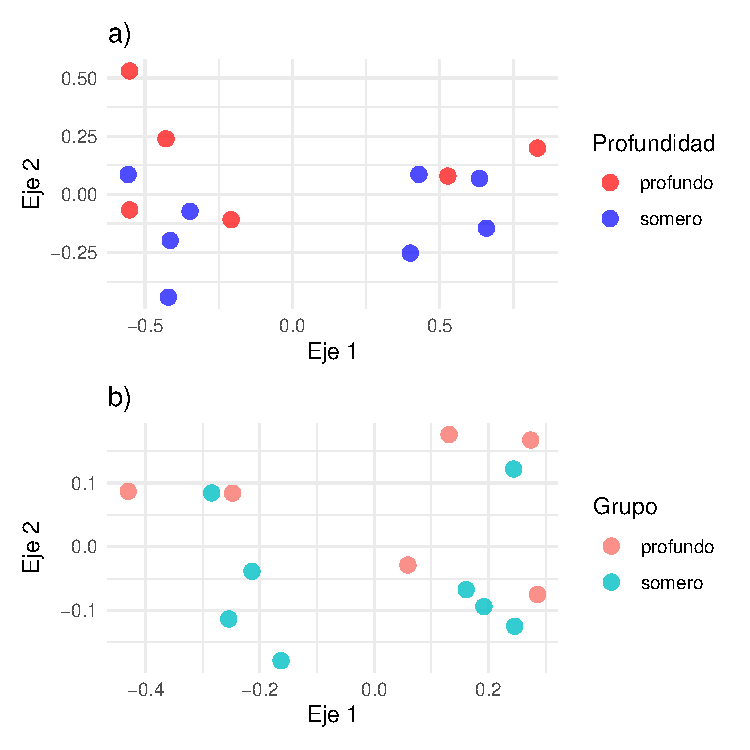
\includegraphics[width=0.5\textwidth,height=\textheight]{ECVI_files/figure-pdf/fig-1-1.pdf}

}

\caption{\label{fig-1}(a) MDS y (b) PCO de la cobertura de la comunidad
de pastos, los colores representan la profundidad (profundo = rojo,
somero = azul).}

\end{figure}%

\begin{longtable}[t]{>{\raggedright\arraybackslash}p{0.7cm}>{\raggedright\arraybackslash}p{0.7cm}>{\raggedright\arraybackslash}p{0.7cm}>{\raggedright\arraybackslash}p{0.7cm}>{\raggedright\arraybackslash}p{0.7cm}>{\raggedright\arraybackslash}p{0.7cm}>{\raggedright\arraybackslash}p{0.7cm}>{\raggedright\arraybackslash}p{0.7cm}>{\raggedright\arraybackslash}p{0.7cm}}

\caption{\label{tbl-2}La cobertura promedio de los cuadrantes en las dos
profundidades, y el total de ambas profundidades por especie. La columna
``Total'' muestra la suma total de los porcentajes de cobertura de todas
las especies. La fila de aporte a la disimilitud muestra cuando las
especies contribuyen a la diferencia entre ambas zonas. Los valores
\emph{p} fueron calculados con la función de simper \{vegan\}, y valores
mas bajos indican un mayor aporte a las diferencias entre las dos
profundidades.}

\tabularnewline

\toprule
\begingroup\fontsize{5}{7}\selectfont Prof\endgroup & \begingroup\fontsize{5}{7}\selectfont S. f.\endgroup & \begingroup\fontsize{5}{7}\selectfont H. b.\endgroup & \begingroup\fontsize{5}{7}\selectfont T. t.\endgroup & \begingroup\fontsize{5}{7}\selectfont L. p.\endgroup & \begingroup\fontsize{5}{7}\selectfont H. i.\endgroup & \begingroup\fontsize{5}{7}\selectfont A. c.\endgroup & \begingroup\fontsize{5}{7}\selectfont P. c.\endgroup & \begingroup\fontsize{5}{7}\selectfont Total\endgroup\\
\midrule
\begingroup\fontsize{5}{7}\selectfont Somero\endgroup & \begingroup\fontsize{5}{7}\selectfont 27.20\%\endgroup & \begingroup\fontsize{5}{7}\selectfont 14\%\endgroup & \begingroup\fontsize{5}{7}\selectfont 10.70\%\endgroup & \begingroup\fontsize{5}{7}\selectfont 28.50\%\endgroup & \begingroup\fontsize{5}{7}\selectfont 12.10\%\endgroup & \begingroup\fontsize{5}{7}\selectfont 2\%\endgroup & \begingroup\fontsize{5}{7}\selectfont 0\%\endgroup & \begingroup\fontsize{5}{7}\selectfont 94.50\%\endgroup\\
\begingroup\fontsize{5}{7}\selectfont Profundo\endgroup & \begingroup\fontsize{5}{7}\selectfont 28.40\%\endgroup & \begingroup\fontsize{5}{7}\selectfont 37.30\%\endgroup & \begingroup\fontsize{5}{7}\selectfont 2.50\%\endgroup & \begingroup\fontsize{5}{7}\selectfont 16.20\%\endgroup & \begingroup\fontsize{5}{7}\selectfont 8.50\%\endgroup & \begingroup\fontsize{5}{7}\selectfont 0.50\%\endgroup & \begingroup\fontsize{5}{7}\selectfont 0.03\%\endgroup & \begingroup\fontsize{5}{7}\selectfont 93.40\%\endgroup\\
\begingroup\fontsize{5}{7}\selectfont Ambos\endgroup & \begingroup\fontsize{5}{7}\selectfont 27.80\%\endgroup & \begingroup\fontsize{5}{7}\selectfont 25.65\%\endgroup & \begingroup\fontsize{5}{7}\selectfont 6.60\%\endgroup & \begingroup\fontsize{5}{7}\selectfont 22.35\%\endgroup & \begingroup\fontsize{5}{7}\selectfont 10.30\%\endgroup & \begingroup\fontsize{5}{7}\selectfont 1.25\%\endgroup & \begingroup\fontsize{5}{7}\selectfont 0.02\%\endgroup & \begingroup\fontsize{5}{7}\selectfont 93.95\%\endgroup\\
\begingroup\fontsize{5}{7}\selectfont Aporte a la disimilitud\endgroup & \begingroup\fontsize{5}{7}\selectfont 0.833\endgroup & \begingroup\fontsize{5}{7}\selectfont 0.069\endgroup & \begingroup\fontsize{5}{7}\selectfont 0.739\endgroup & \begingroup\fontsize{5}{7}\selectfont 0.317\endgroup & \begingroup\fontsize{5}{7}\selectfont 0.888\endgroup & \begingroup\fontsize{5}{7}\selectfont 0.43\endgroup & \begingroup\fontsize{5}{7}\selectfont 0.23\endgroup & \begingroup\fontsize{5}{7}\selectfont NA\endgroup\\
\bottomrule

\end{longtable}

\begin{figure}

\centering{

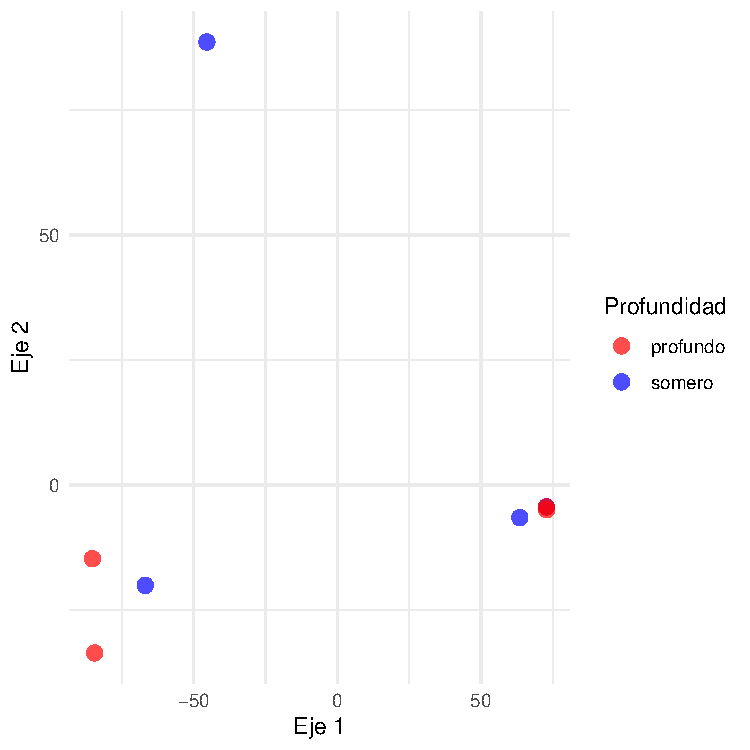
\includegraphics[width=0.5\textwidth,height=\textheight]{ECVI_files/figure-pdf/fig-2-1.pdf}

}

\caption{\label{fig-2}MDS del peso de las algas extraídas de un
cuadrante de 25 cm\^{}2. Los muestreos en zonas profundas están
representados por los puntos rojos mientras los de las zonas someras en
azul.}

\end{figure}%

Para el protocolo de biomasa de algas se colectaron las algas de 8 SUM.
Se identificaron 7 especies, 4 de las cuales no se habían presentado en
el muestreo de cobertura (\emph{Dictyota divaricata}, \emph{Dictyota
cervicornis}, \emph{Udotea sp.}, \emph{A. crenulata}). El PERMANOVA no
mostró diferencias significativas entre las dos profundidades (F =
1.4239, \emph{p = 0.2621}). Por último se habían extraído 8 núcleos de
sedimento. Ninguno de los análisis a los datos extraídos de los núcleos
mostraron diferencias significativas (biomasa de las algas y pastos, F =
0.6667, \emph{p = 0.7119}; número de haces, F = 0.4803, \emph{p =
0.7418}; individuos más largos, F = 1.4908, \emph{p = 0.2837}).

\subsection{Peces}\label{peces-1}

Las cámaras trampa capturaron un total de 1,514 fotos, 39 de las cuales
contenían peces. Se lograron identificar dos especies. La especie que
más salió en las fotos fue \emph{Eucinostomus gula} (mojarra española),
es probable que las distintas fotos sean del mismo individuo
(Figure~\ref{fig-3}) La segunda especie que se logró identificar fue
\emph{Sphoeroides testudineus}, que apareció en solamente una imagen
(Figure~\ref{fig-4}). Hubo una imagen que capturó a 4 peces pero por la
distancia a la cámara no se lograron identificar.

\begin{figure}

\centering{

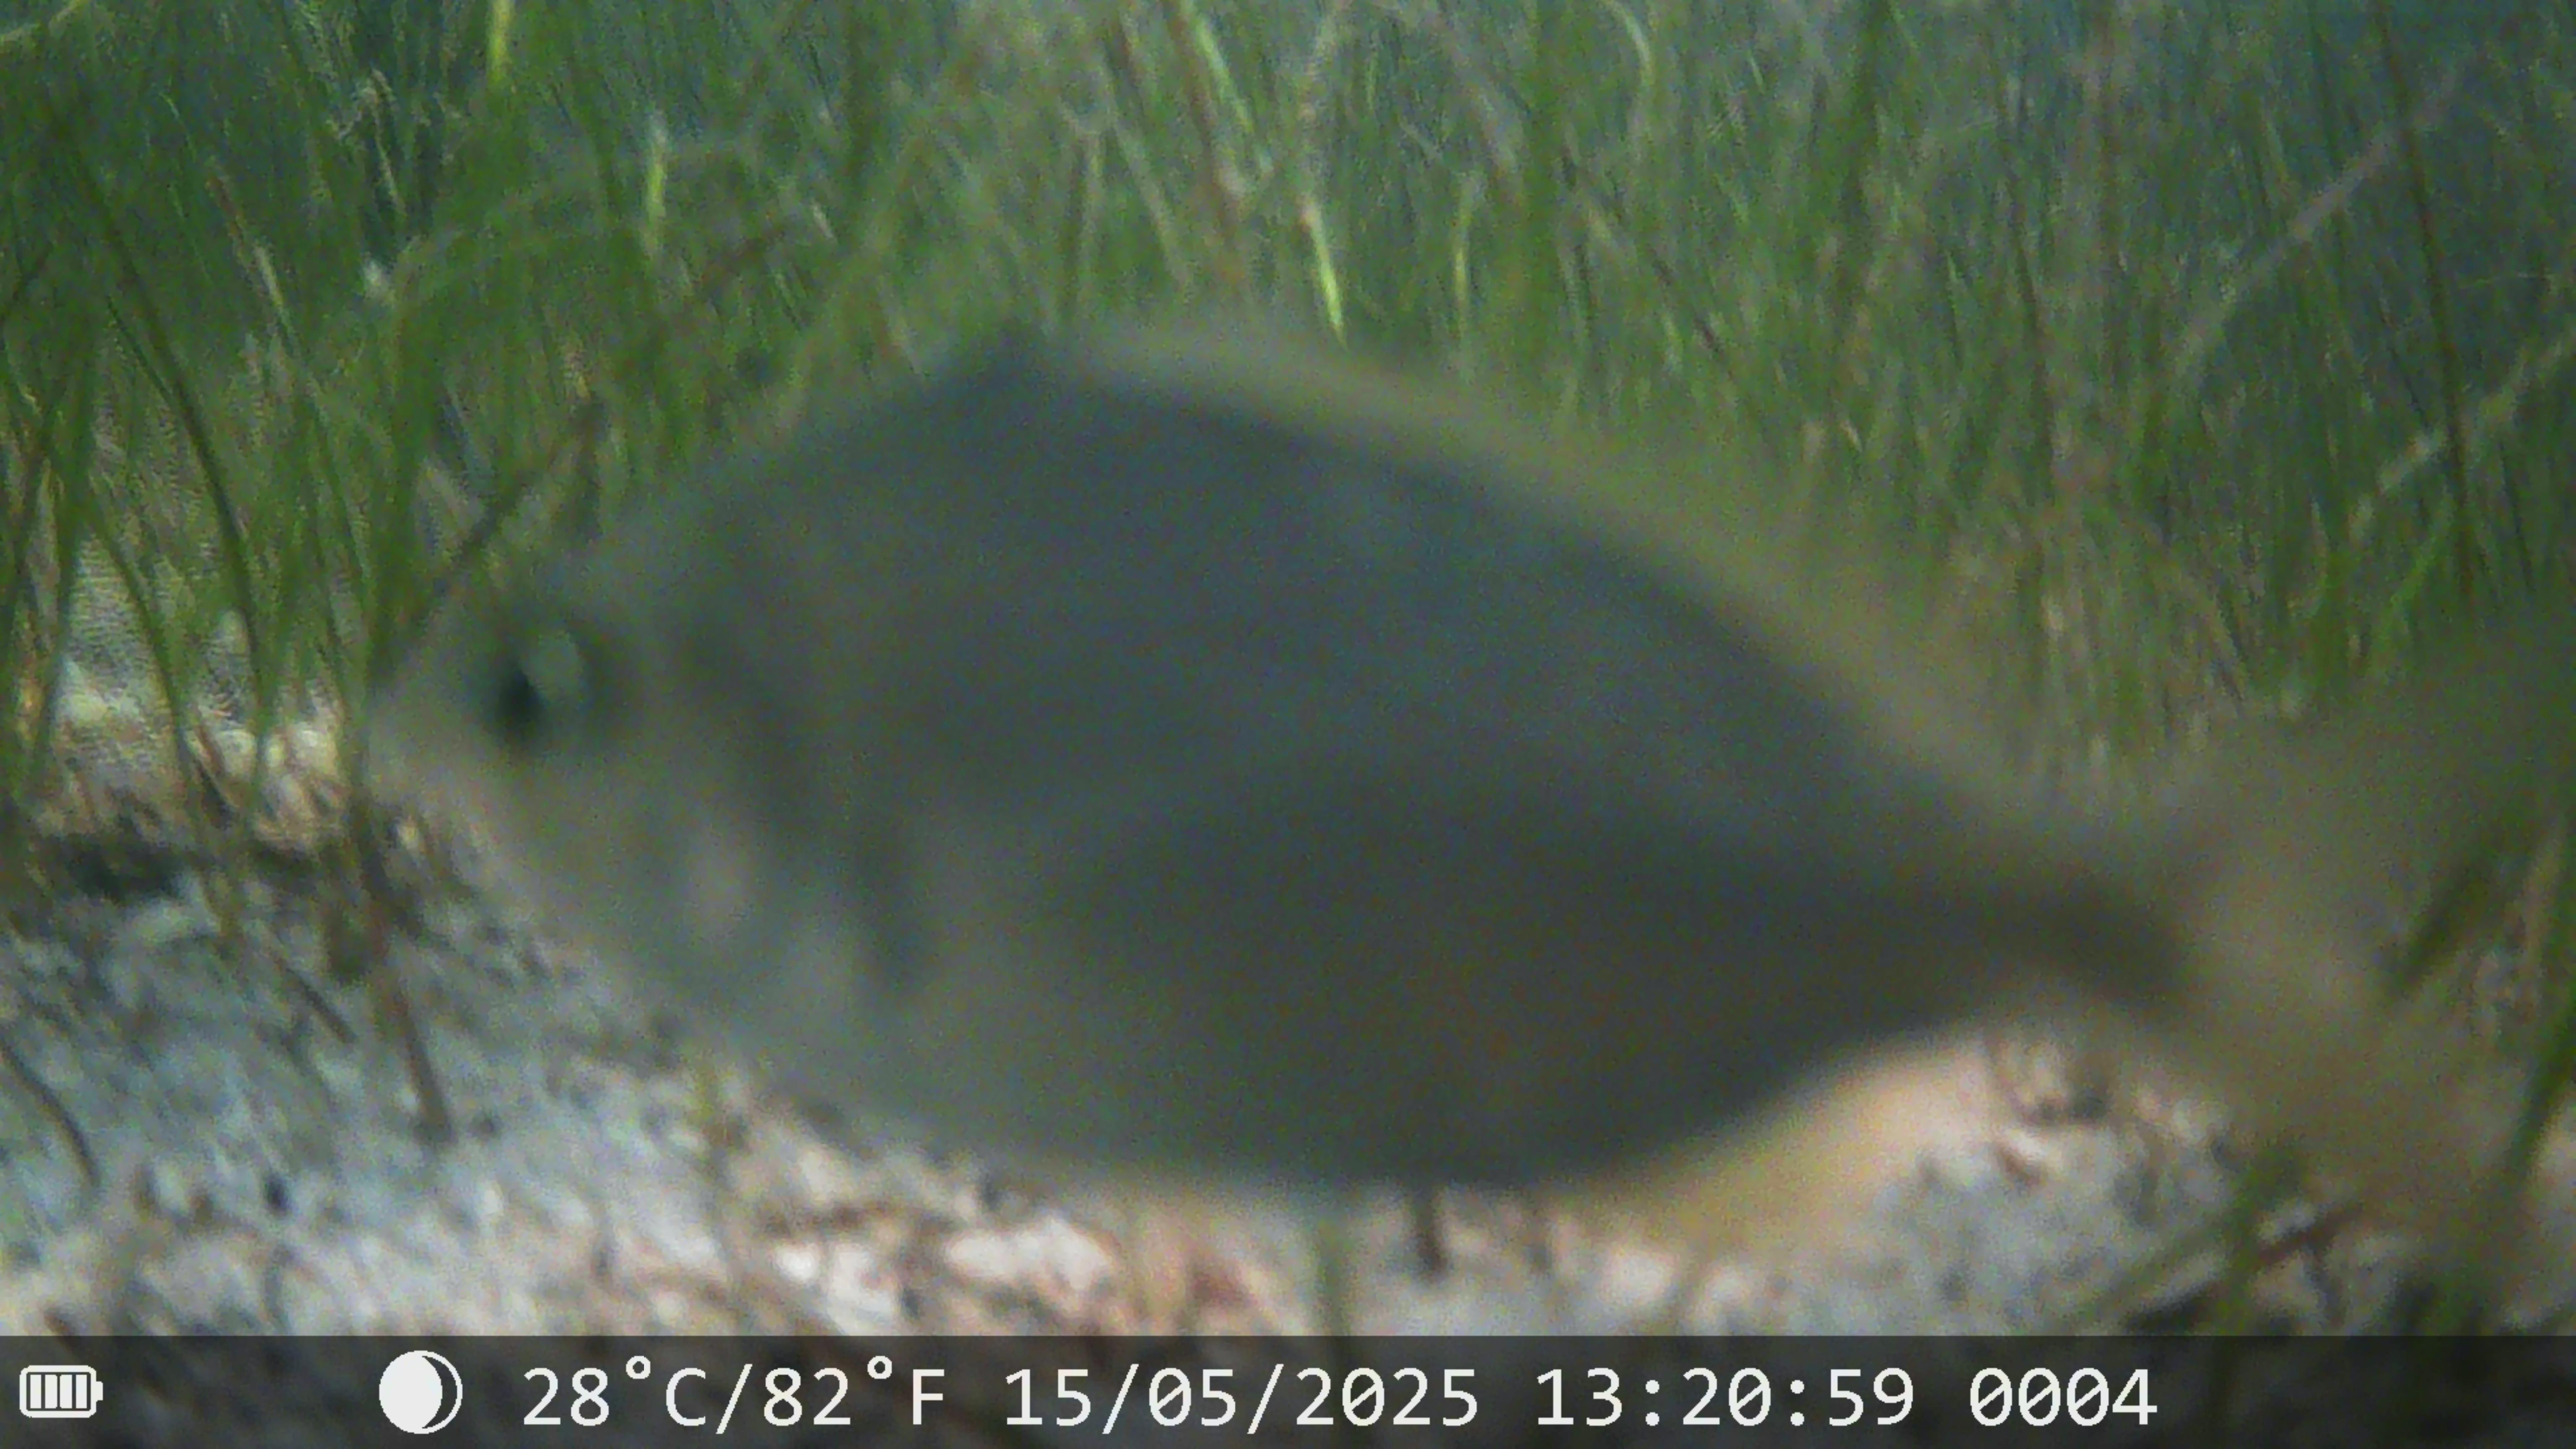
\includegraphics[width=0.5\textwidth,height=\textheight]{FOTOS/DSCF0173_Egula.JPG}

}

\caption{\label{fig-3}Foto capturada con la cámara trampa de \emph{E.
gula}.}

\end{figure}%

\begin{figure}

\centering{

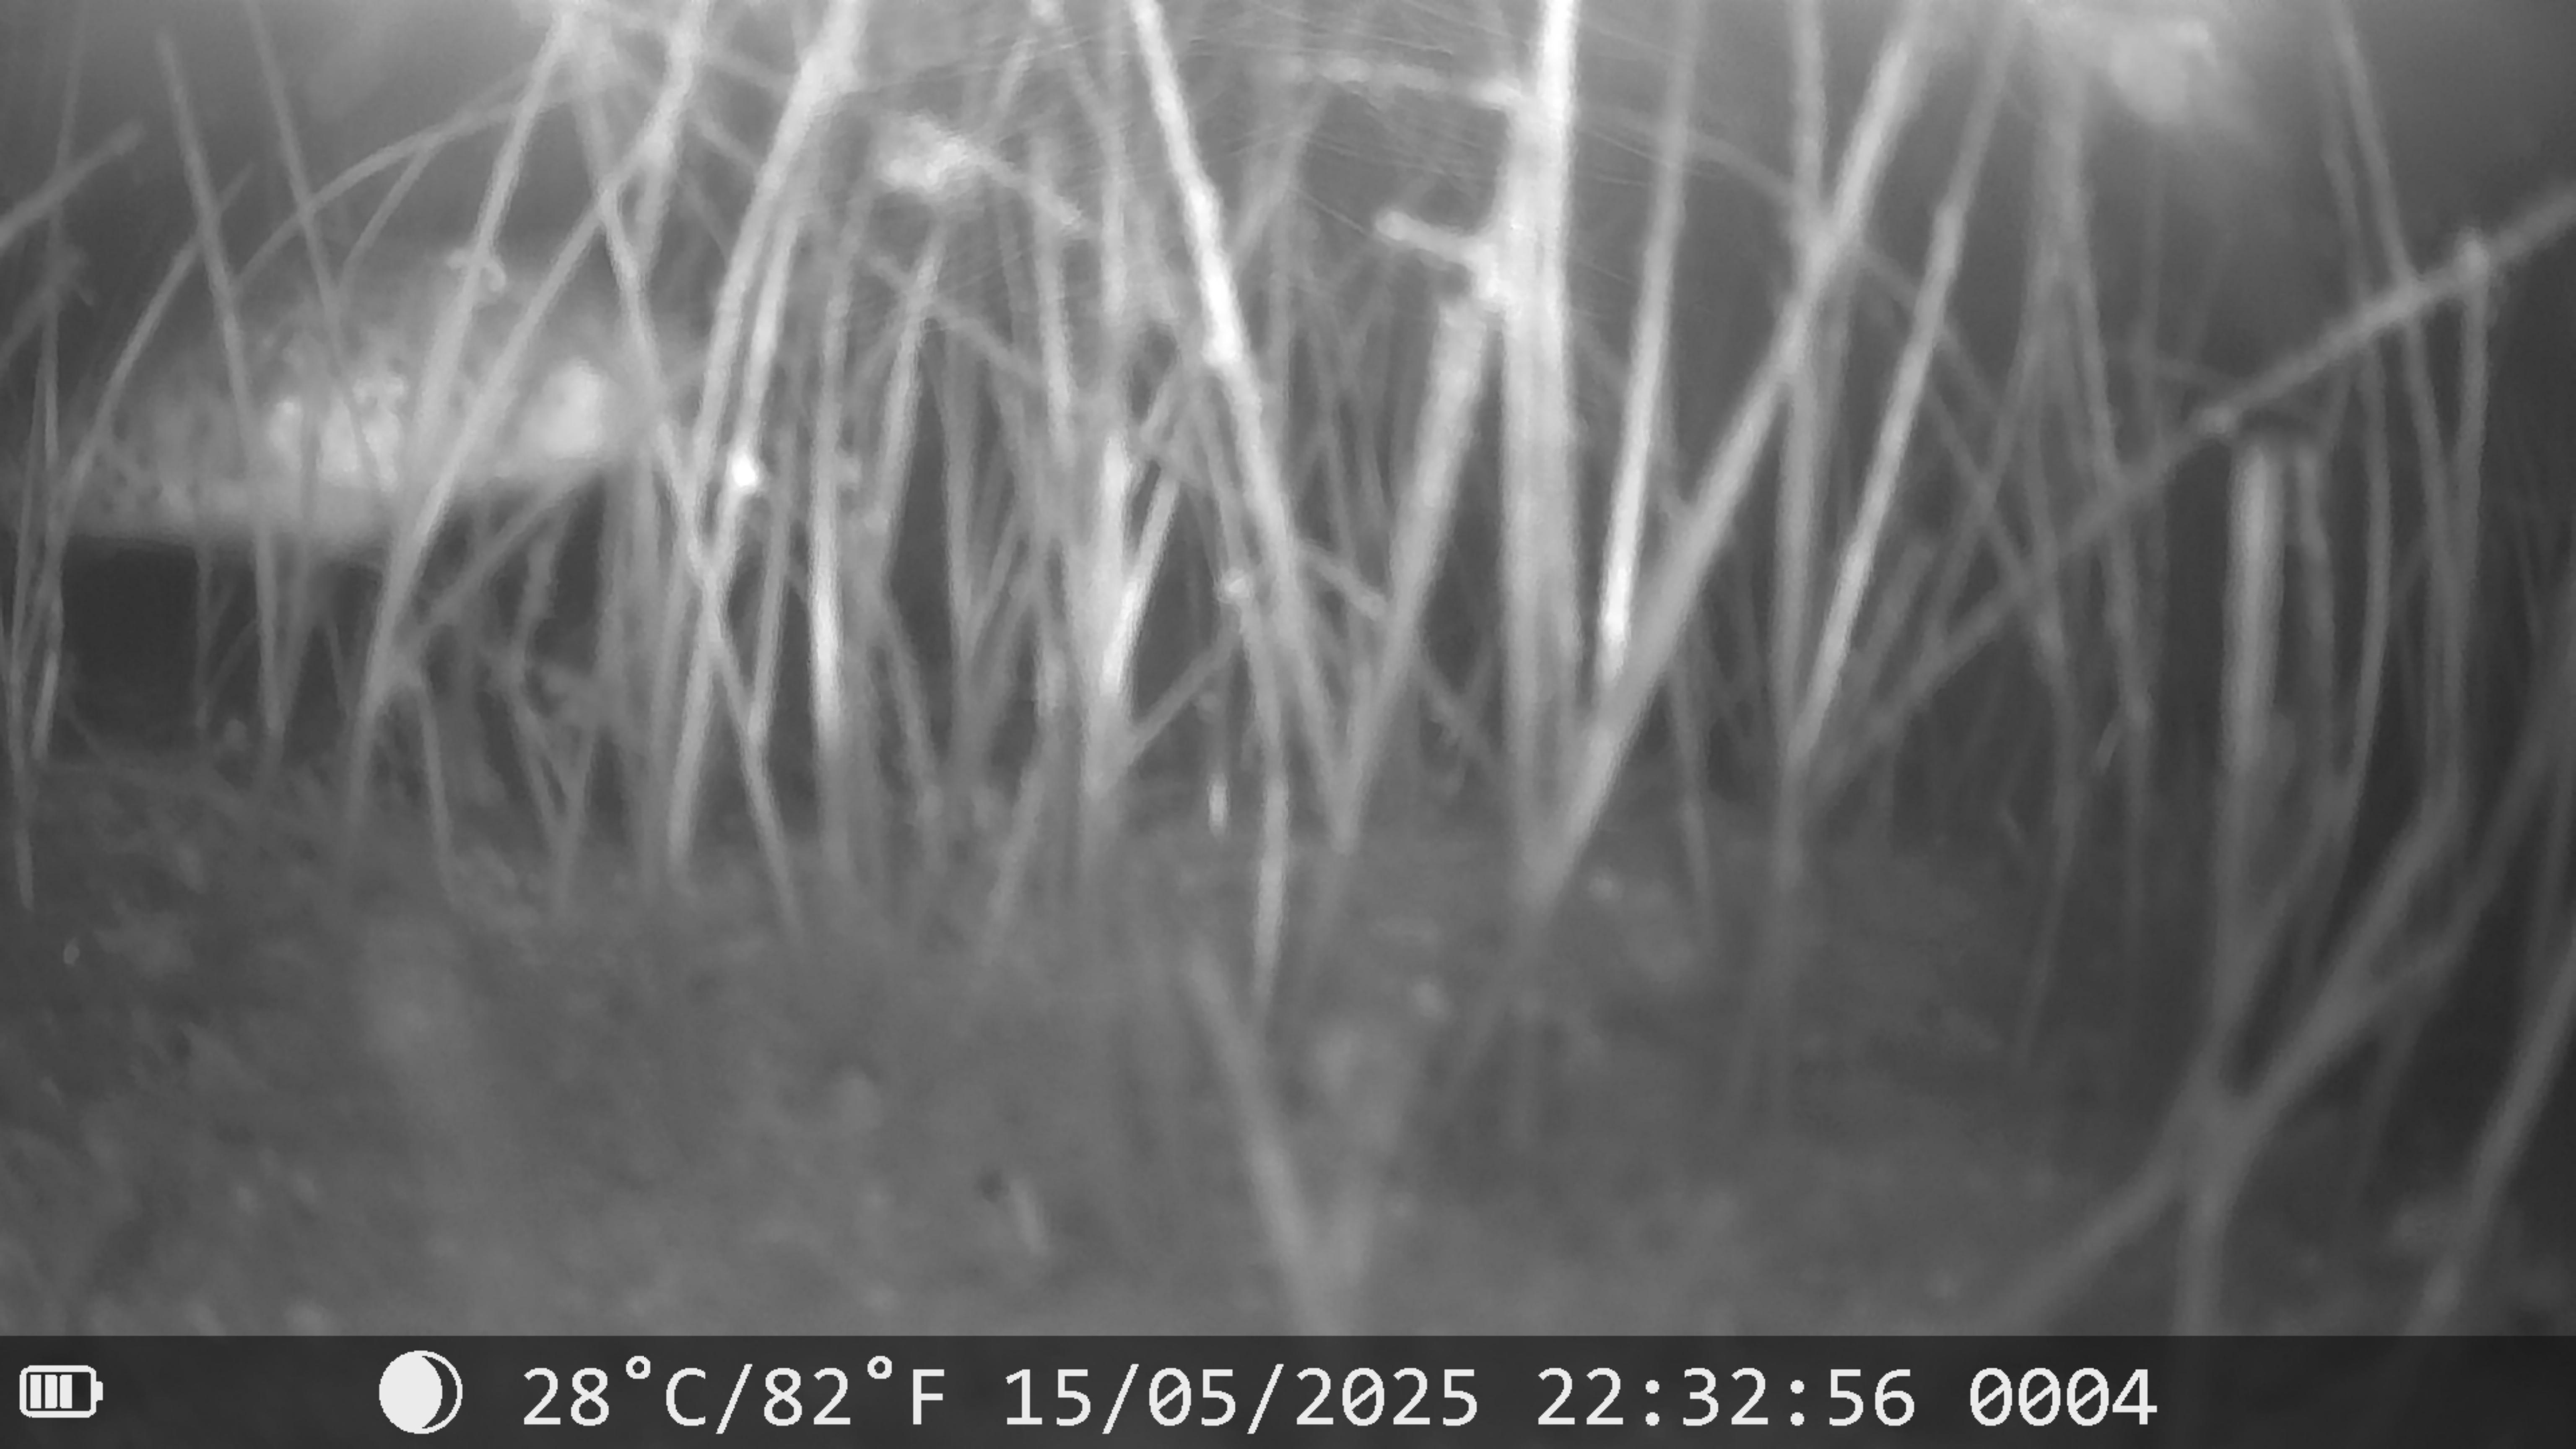
\includegraphics[width=0.5\textwidth,height=\textheight]{FOTOS/DSCF0450_S.JPG}

}

\caption{\label{fig-4}Foto capturada con la cámara trampa de \emph{S.
testudineus}.}

\end{figure}%

\subsection{Oligoquetos}\label{oligoquetos-1}

Durante el transcurso de la práctica se realizaron 8 transectos, 4 en el
horario matutino y en el horario vespertino. En cada transecto se
extrajeron 9 núcleos: 4 en la zona submareal, 1 en el intermareal, y 4
en la área supramareal. En total se realizaron 72 muestreos donde se
recolectaron 1,226 oligoquetos con un tamaño medio de 4.5 cm, una
mediana de 3.8, con un rango en tamaño de entre 0.2 cm y 20.1 cm. La
abundancia de individuos por núcleo estuvo entre 0 y 141, con una media
de 15.8 y mediana de 3. La mayoría de oligoquetos se encontraron al
centro del transecto, con los muestreos en el supramareal 4 y submareal
4, sin presentar ningún oligoqueto en la mayoría de los muestreos. Para
ambas variables los muestreos más alejados del intermareal, tanto en las
zonas submareales, como las supramareales, presentaron valores medios
más bajos.

\begin{figure}

\centering{

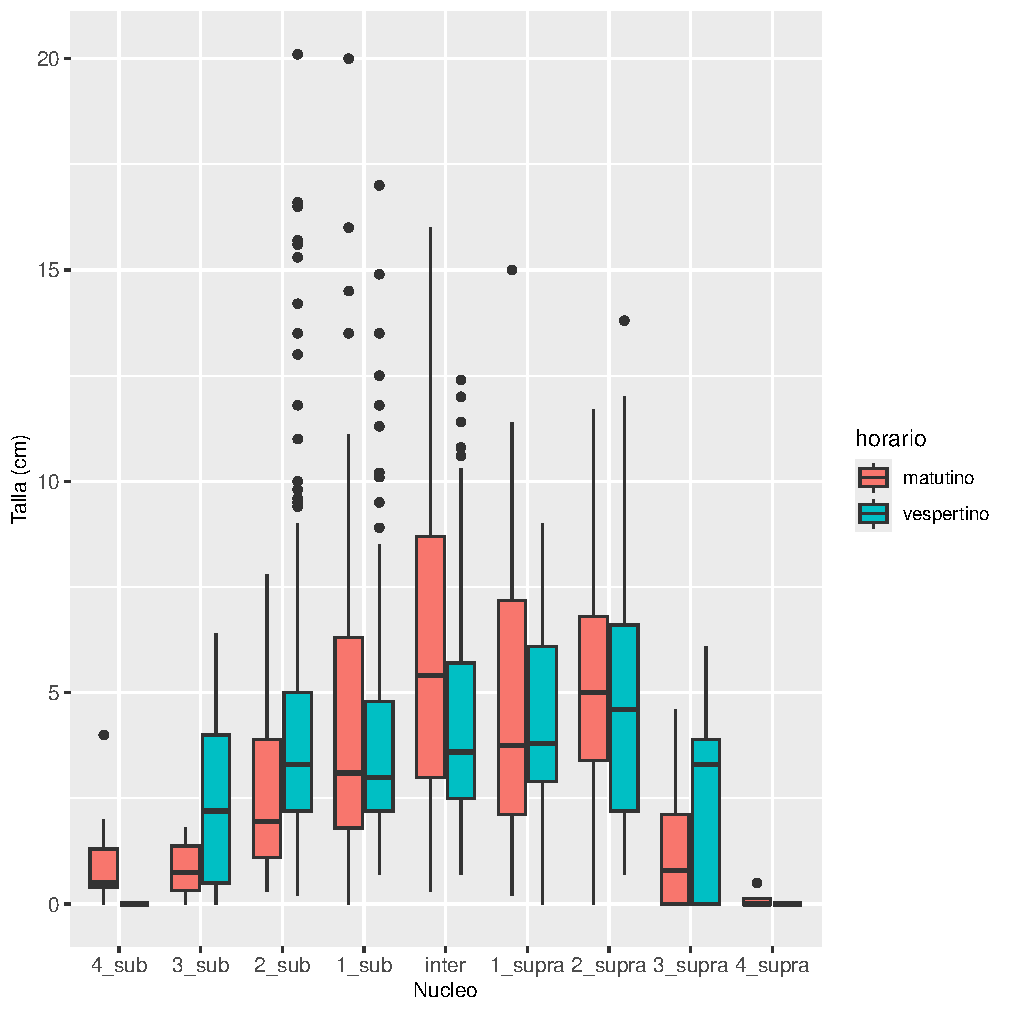
\includegraphics[width=0.5\textwidth,height=\textheight]{ECVI_files/figure-pdf/fig-5-1.pdf}

}

\caption{\label{fig-5}Boxplot de la talla de oligoquetos en los
distintos muestreos de la playa. Los colores representan horarios
distintos (matutino = rojo, vespertino = azul).}

\end{figure}%

\begin{figure}

\centering{

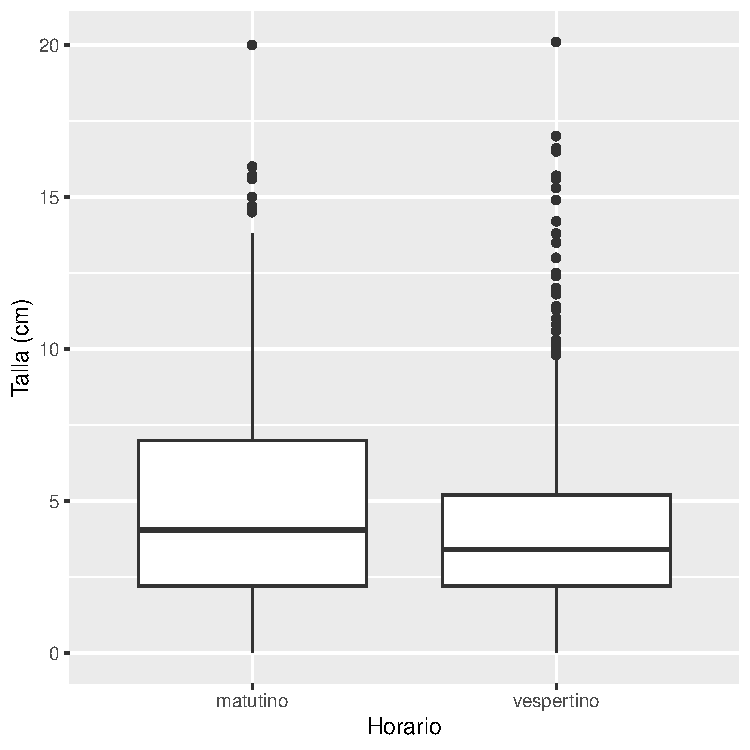
\includegraphics[width=0.5\textwidth,height=\textheight]{ECVI_files/figure-pdf/fig-6-1.pdf}

}

\caption{\label{fig-6}Boxplot de la talla de oligoquetos en ambos
horarios.}

\end{figure}%

\begin{figure}

\centering{

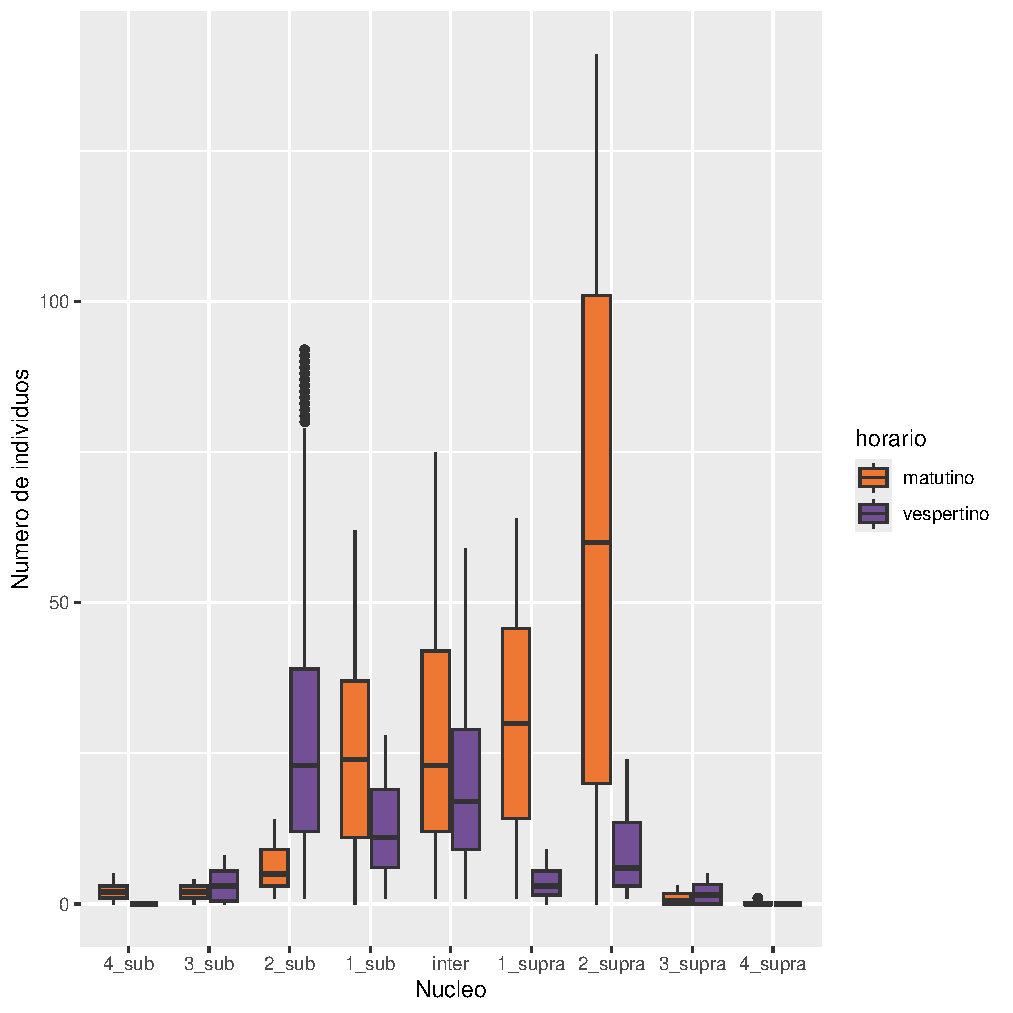
\includegraphics[width=0.5\textwidth,height=\textheight]{ECVI_files/figure-pdf/fig-7-1.pdf}

}

\caption{\label{fig-7}Boxplot de la abundancia de oligoquetos a lo largo
de los transectos. Los colores representan el horario (matutino = rojo,
vespertino = morado).}

\end{figure}%

El análisis mostró que tanto la hora (F = 10.081, \emph{p \textless{}
0.01}; Figure~\ref{fig-6}), como la posición en la playa (F = 51.336 ,
\emph{p \textless{} 0.01}; Figure~\ref{fig-5}) y la interacción entre
ambos (F = 28.042, \emph{p \textless{} 0.01}), son factores que influyen
de manera significativa sobre la talla. El tamaño promedio de los
oligoquetos extraídos en el horario matutino es ligeramente mayor que
los encontrados en el horario vespertino. El tamaño de los oligoquetos
va incrementando desde el submareal 4 hasta el intermareal donde se
mantiene constante hasta el supramareal 2 donde vuelve a declinar. Para
la variable de abundancia únicamente la posición en la playa influyó de
manera significativa (F = 10.554, \emph{p = 0.0001};
Figure~\ref{fig-7}), sin embargo la interacción entre las dos variables
fue significativa. Para ambas variables los muestreos más alejados del
intermareal, tanto en las zonas submareales, como las supramareales,
presentaron valores medios más bajos.

\section{Discusión}\label{discusiuxf3n}

Este estudio analiza el estado ecológico de una playa representativa de
la península de Yucatán, centrándose en tres grupos de organismos clave
para el ecosistema, involucrados en la salud de la comunidad a través de
sus interacciones bióticas. Con base en los resultados obtenidos de los
análisis, no podemos afirmar con certeza que nuestras predicciones
iniciales se hayan cumplido, pero tampoco podemos descartarlas por
completo, ya que se observa una tendencia acorde con lo planteado, aún
si los datos obtenidos no ofrecen evidencia suficiente para confirmar
que las predicciones se cumplieron. Para futuras investigaciones,
sugerimos aumentar la cantidad de muestras para obtener datos más
representativos y mejorar la precisión de los análisis.

Estudios previos han señalado una abundante presencia de organismos
intersticiales tanto en la zona intermareal como en la supramareal,
particularmente en regiones húmedas pero no sumergidas,
\citet{McLachlanBrown2006} denominaron este espacio como la ``zona de
retención''. De la misma manera, la distribución de estos organismos,
debido a su carácter de menores dimensiones, está influenciada
principalmente por interacciones bióticas, como la atracción para la
reproducción y la evasión de depredadores \citep{Giere2009}.

Así, el constante movimiento de las corrientes marinas resulta
fundamental en esta distribución, pues se ha observado que el
levantamiento del sedimento los deja expuestos y vulnerables a sus
depredadores y a ser transportados incluso por corrientes de baja
intensidad, lo que limita su permanencia en zonas de inundación
prolongada \citep{McLachlanBrown2006}. Para estudios futuros, será
esencial considerar la influencia de las variaciones en la altura de la
marea en la distribución de estas poblaciones, en lugar de asumir un
punto fijo como zona intermareal.

La distribución de oligoquetos sigue patrones definidos, aunque con
ciertas variaciones irregulares. \citet{EdwardsArancon2022} reportan
ritmos de actividad diurnos, lo que indica que los horarios en los que
se realizaron los muestreos no fueron la causa de la falta de
certidumbre en los datos. Además, el número de individuos por núcleo fue
similar con lo reportado previamente en estudios que utilizaron la misma
metodología en la misma zona \citep{Guerra-Castro2020}, lo que sugiere
que los datos obtenidos son representativos de la población estudiada.

Por otra parte, durante el muestreo, se registró una cobertura de
biomasa de vegetación en descomposición sobre la zona de retención en la
supramareal, lo que pudo haber influido en la retención de humedad del
ambiente intersticial y, en consecuencia, en la distribución de la
población de \emph{T. diazi} en la playa. Estos factores pudieron haber
sido la causa de que los datos no fueran lo suficientemente contundentes
para respaldar con certeza los fenómenos previamente descritos, por lo
tanto, representan un punto de partida para futuras investigaciones que
consideren estos elementos.

En cuanto al registro de peces, las cámaras utilizadas para la grabación
no estaban correctamente configuradas, lo que impidió la obtención de
datos. Respecto a las fotografías, el material obtenido no representa la
diversidad reportada previamente en la zona, la cantidad de especies que
reportamos sólo cubre 2 de las 81 reportadas para la comunidad de la
localidad, sin embargo, son dos de las seis especies más abundantes en
el sitio \citep{ArceoCarranza2009}.

Para futuros trabajos de monitoreo recomendamos seguir la metodología de
\citet{ArceoCarranza2009}, donde se llevaron a cabo seis muestreos
bimestrales, separados por dos meses, que en conjunto abarcaron un
período de un año. Un monitoreo más prolongado permitirá observar una
mayor y mejor representación de la fauna íctica de la región y el papel
de la comunidad de pastos marinos como zonas de gran impacto ecológico
\citep{CATALAN_DUNAND_ÁLVAREZ_ALOS_COLINAS_NASH_2014}.

Por otro lado, para la evaluación del desarrollo de la composición de
pastos marinos tampoco observamos datos contundentes para asegurar el
cumplimiento de nuestras predicciones, sin embargo, como en los casos
anteriores, una ampliación de nuestra metodología permitiría observar
variación de manera más significativa, un mayor número de muestras y
profundidades más alejadas de la línea de la costa. Resaltamos
particularmente los resultados obtenidos para la cobertura, sería
recomendable realizar mediciones adicionales mar adentro, pues, a pesar
de que la distancia a la que llevamos a cabo el muestreo no presentó la
variación esperada, la profundidad, como se observa en la
Figure~\ref{fig-1}, explica en buena medida dicha variación, aunque no
la explique lo suficiente.

No consideramos que la aparente homogeneidad de la comunidad de pastos
marinos sea consecuencia de eventos de origen antrópico o natural, sino
por limitaciones en la metodología empleada. Sin embargo, resaltamos la
importancia de considerar ciertas perturbaciones en futuros estudios
dirigidos a evaluar y reportar el estado ecológico de las comunidades
costeras.

\citet{HERRERASILVEIRA200972} reportan que los cambios negativos en la
cobertura y composición de especies de vegetación acuática sumergida en
pastos marinos están generalmente asociados con la eutrofización del
ambiente \citep{OrthMoore1983, Stevenson1993}, provocada por un
crecimiento excesivo de macroalgas y epífitas \citep{Dennison1993}; así
mismo, indican que no existe una medida que determine cuándo el
crecimiento de estos organismos se vuelve nocivo para la comunidad. No
obstante, resaltan que un buen acercamiento para evaluar esta situación
es examinar el cambio en el porcentaje de cobertura en el tiempo
\citep{Bricker2003}. Así, llevar a cabo monitoreos periódicos siguiendo
una metodología estandarizada, se vuelve clave para prevenir el
deterioro en la salud de la comunidad de pastos marinos.

Por otra parte, \citet{Herrera-Silveira2019} analizan el impacto de los
puertos industrializados en las comunidades de pastos marinos,
especialmente en zonas de intenso desarrollo costero, donde la pérdida
de extensas áreas de estas plantas ocurre a un ritmo acelerado. De la
misma manera, presentan los efectos de estas pérdidas en la calidad del
agua, como el aumento de la turbidez debido a la disminución en la
retención de sedimentos y la eutrofización causada por la ausencia de
estos organismos clave en el ciclaje de nutrientes.

Además, las comunidades de pastos marinos también se ven afectadas por
eventos hidrometeorológicos, los cuales incrementan la escorrentía y, en
consecuencia, la turbidez del agua, reduciendo la disponibilidad de luz.
Este fenómeno se agrava en el caso de tormentas prolongadas, que pueden
durar semanas y causar daños significativos, al dañar, remover y
enterrar grandes cantidades de biomasa de estas plantas acuáticas
\citep{Herrera-Silveira2019}.

Aunque nuestro estudio no obtuvo evidencia concluyente para determinar
el estado ecológico de la comunidad en la playa de Dzilam de Bravo, sí
ofrece un panorama sobre las condiciones en las que se encuentra. En
zonas como esta, donde las comunidades de pastos marinos están sometidas
a una intensa presión por efectos antrópicos derivados de grandes
desarrollos costeros, así como por factores naturales propios de una
región expuesta constantemente a eventos hidrometeorológicos, es
fundamental realizar muestreos periódicos y estandarizados que permitan
evaluar el impacto de dichas perturbaciones en los pastos marinos, zonas
clave para garantizar la sostenibilidad y el bienestar de las
comunidades costeras y marinas, regionales y globales, al ser sitios
esenciales para la interacción intra e interespecífica.


\renewcommand\refname{Referencias}
  \bibliography{bibliography.bib}



\end{document}
